%!TEX root = Slic3r-Manual.tex
\section{Mode Simple} % (fold)
\label{sec:simple_mode}
\index{simple mode}
\index{mode simple}

Slic3r a deux modes de fonctionnement, Simple et Expert. Ceux-ci peuvent être choisis à partir de la fenêtre \texttt{Preferénces} (qui se trouve dans le menu  \texttt{File} (fichier) ).

\begin{figure}[ht]
\centering
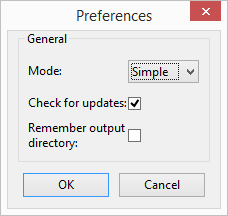
\includegraphics[width=0.3\textwidth]{simple_mode/preferences_general.png}
\caption{Preférences.}
\label{fig:preferences_general}
\end{figure}

Le mode simple offre une gamme réduite de paramètres, suffisament pour que le débutant puisse commencer. Le mode expert donne plus de contrôle sur la manière dont Slic3r produit le G-code, celui-ci sera examiné plus tard.

\subsection{Paramètres d'Impression}
\index{Print Settings}
\index{paramètres d'impression}

L'onglet \texttt{Print Settings} (paramètres d'impression) 
offre la possibilité de modifier les paramètres liés à l'impression réelle. Alors que les autres onglets sont modifiées moins souvent, les paramètres de cet onglet seront modifiés régulièrement, éventuellement pour chaque modèle imprimé.

\begin{figure}[ht]
\centering
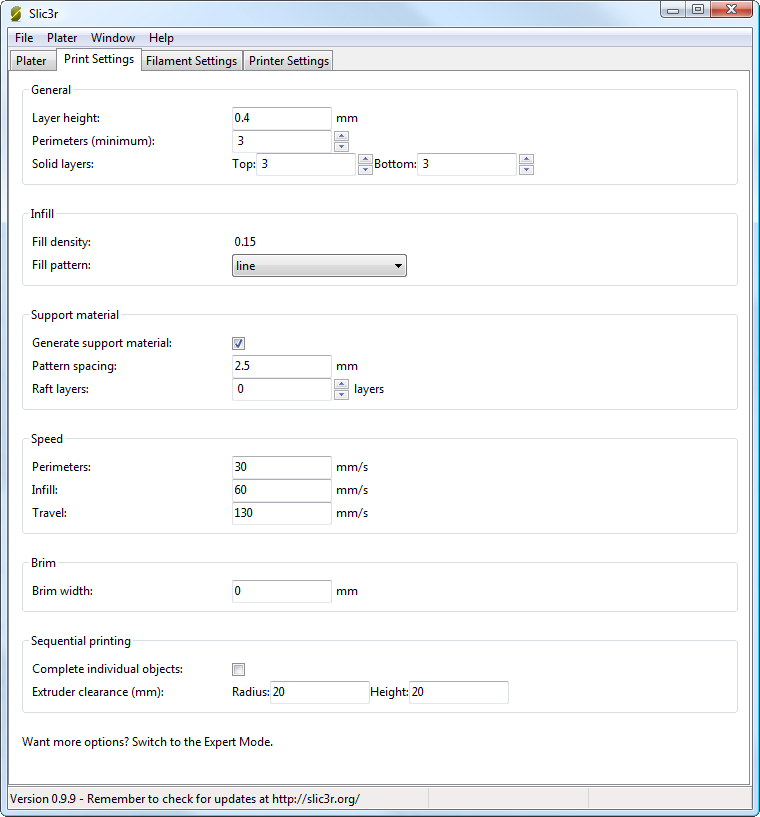
\includegraphics[width=\textwidth]{simple_mode/simple_mode_print_settings.png}
\caption{Mode Simple: Paramètres d'impression.}
\label{fig:simple_mode_print_settings}
\end{figure}

\paragraph{Général.} % (fold)
\label{par:simple_general}
\index{Print Settings!Layer height}
\index{Paramètres d'impression!Epaisseur de couche}

\texttt{Layer height} (épaisseur de couche) définit le déplacement sur l'axe vertical avant l'extrusion d'une nouvelle couche.  Il y a plusieurs facteurs qui influentsur la hauteur que la couche doit avoir:
\begin{itemize}
	\item \textbf{Résolution Désirée}  - Une faible hauteur de couche devrait conduire à des impressions avec des nervures ou des bandes moins visibles, comme chaque couche est plus petite. L'esthétique joue ici un rôle, mais aussi le type de modèle, par exemple, une pièce mécanique peut ne pas avoir besoin d'une telle finition haute résolution, alors qu'une pièce de présentation peut en avoir besoin.
	\item \textbf{Vitesse d'impression}  - Les couches plus fines produiront des impression lisses, mais chaque impression prendra plus de temps, tout simplement parce que l'extrudeuse doit tracer le motif plusieurs fois. Un des buts plus tard sera de trouver un équilibre entre la hauteur de couche, la vitesse de l'imprimante, et la qualité de l'impression qui en résulte.
\end{itemize}
\index{Print Settings!Perimeters}
\index{Paramètres d'impression!Périmètres}
\texttt{Perimeters} (Périmetres) définit le nombre minimum de coquilles verticales (c'est à dire les murs) que l'impression aura. À moins que le modèle ne nécessite qu'un seul mur, il est généralement recommandé d'avoir un minimum de deux périmètres car cela donne l'assurance que si une partie du périmètre ne s'imprime pas correctement alors le second périmètre permettra le de couvrir.

\index{Print Settings!Solid layers}
\index{Paramètres d'impression!Couches pleines}
Les couches supérieure et inférieure qui prennent en sandwich le modèle sont remplis de motifs de \texttt{Solid layers} (couches pleines). Pour les couches inférieures (bottom) le facteur important à prendre en compte est la façon dont la surface aura l'air s'il y avait une anomalie, lors de l'impression de la première couche, c'est pour cette raison, qu'il est recommandé d'avoir au moins deux couches inférieures.

Une prise en compte similaire est nécessaire pour les couches supérieures (top). Parce que les couches intermédiaires sont susceptibles d'être rempli d'un motif fixé à moins de 100\% , les couches de revêtement devront combler ce motif et cela peut nécessiter plus d'un passage pour le couvrir complètement.

\begin{figure}[H]
\centering
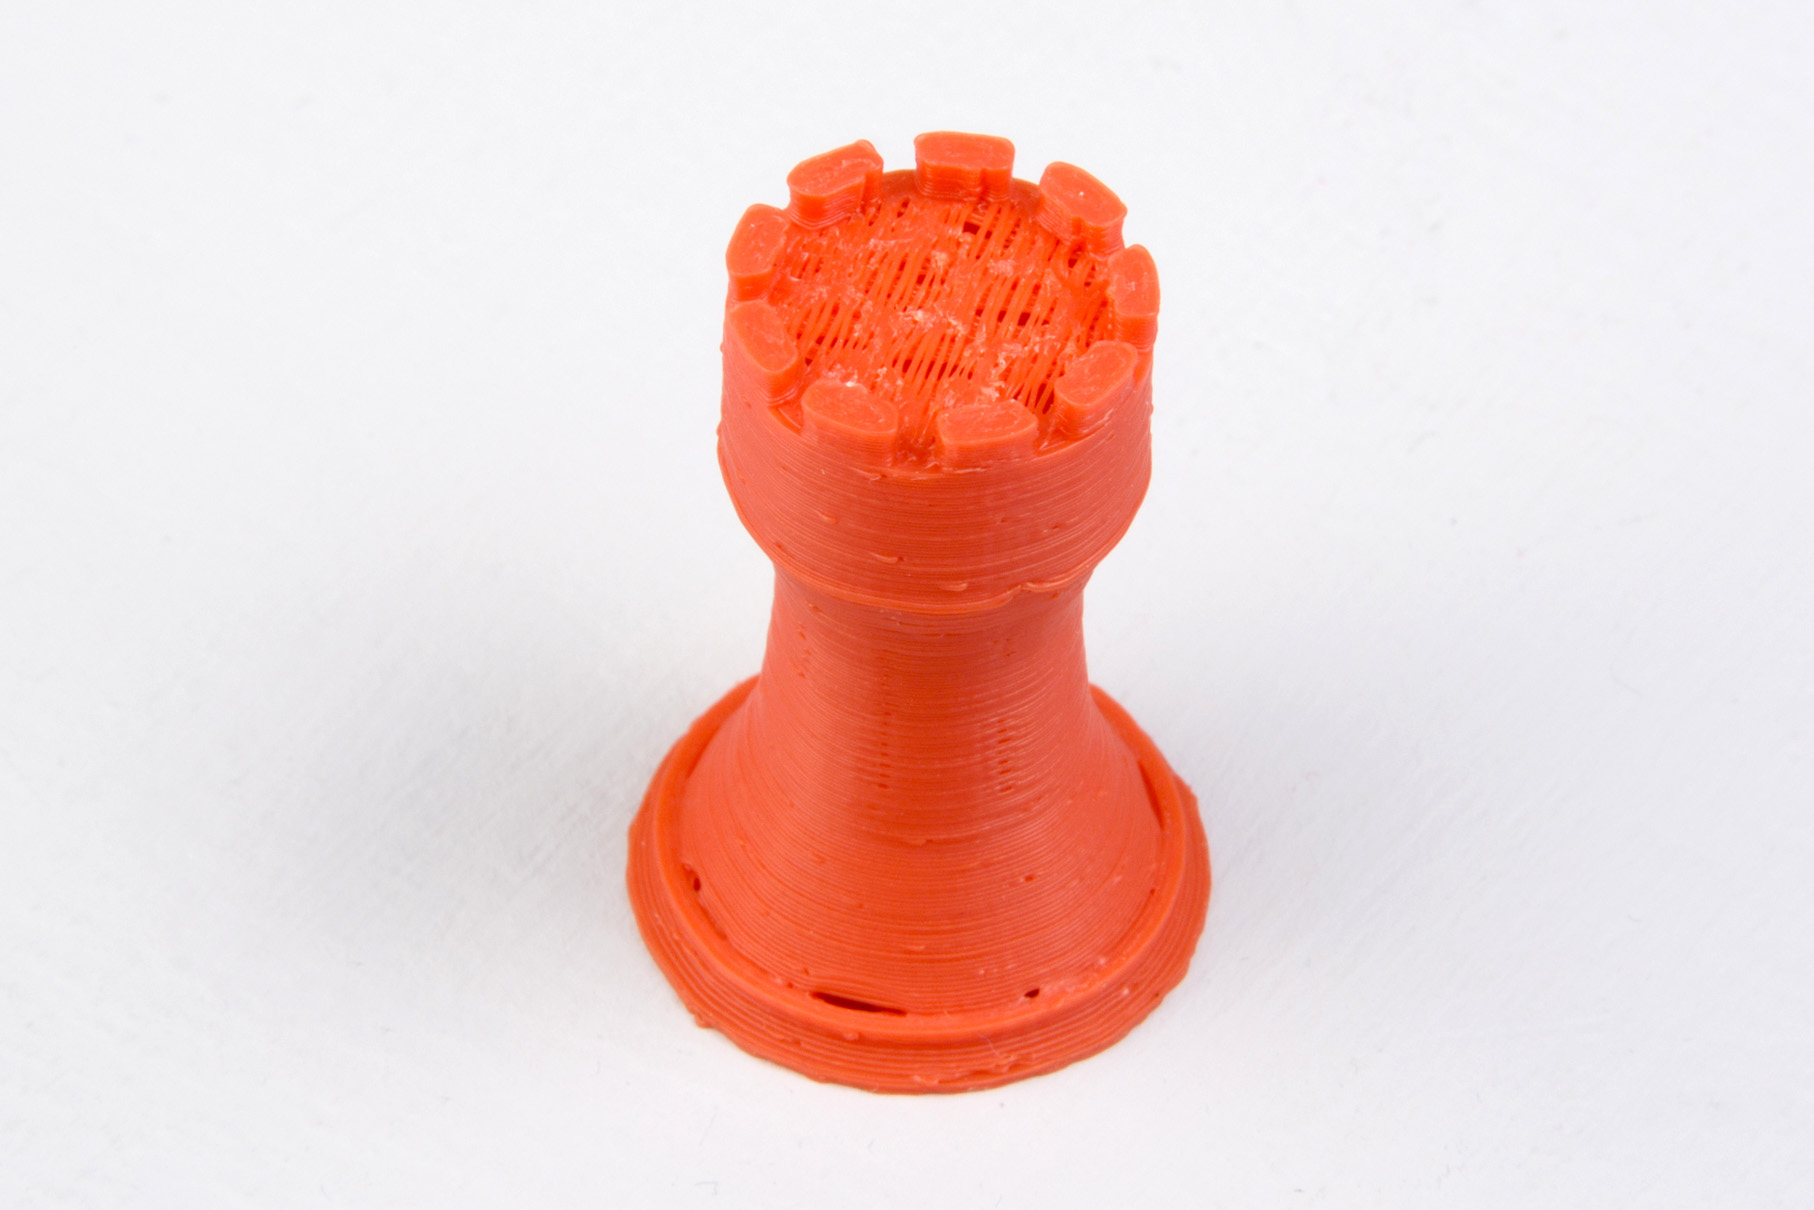
\includegraphics[keepaspectratio=true,width=0.75\textwidth]{simple_mode/bad_top_infill.jpg}
\caption{Un exemple de couches supérieures insuffisantes.}
\label{fig:bad_top_infill}
\end{figure}

Une autre astuce à considérer: Régler la couche pleine supérieure (top solid layer) à zéro, et régler le remplissage également à zéro, produira un récipient , idéal pour transformer les modèles en vases\footnote{http://slic3r.org/blog/tip-printing-vases} par exemple. Ici la modification des paramètres peuvent être utilisés dans Slic3r pour générer différents types de impressions, et pas seulement pour contrôler la précision de surface.

\begin{figure}[H]
\centering
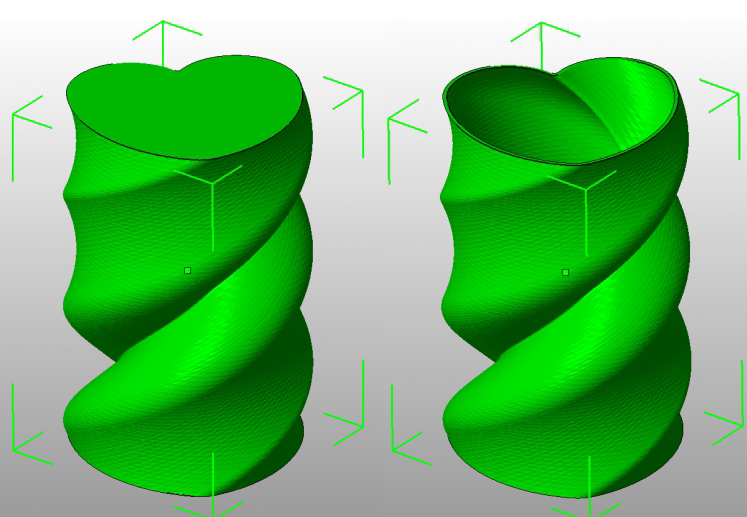
\includegraphics[keepaspectratio=true,width=0.75\textwidth]{simple_mode/solid_layers_vases.png}
\caption{Création d'un vase à partir d'un modèle solide.}
\label{fig:solid_layers_vases}
\end{figure}

% paragraph general (end)

\paragraph{Remplissage. (Infill)} % (fold)
\label{par:simple_infill}
\index{Print Settings!Infill}
\index{Paramètres d'impression!Remplissage}
\index{Print Settings!Infill!Fill density}
\index{paramètres d'impression!Densitée de remplissage}
\texttt{Fill density} (Densité de remplissage) est définie sur une échelle comprise entre 0 et 1, où 1 est de 100\% et 0,4 serait 40\%. Pour la majorité des cas, remplir la pièce à 100\% n'a pas d'intérêt, ce serait un gaspillage de matériel et prendrait beaucoup de temps. Au lieu de cela, la plupart des modèles peuvent être remplis avec moins de matière, qui sera ensuite pris en sandwich entre les couches remplies à 100\% (voir \texttt{Solid layers} au dessus).

Une valeur de densité de 0,4 est suffisant pour donner à la quasi-totalité des modèles une bonne résistance mécanique. Une valeur de 0,2 est généralement le minimum requis pour soutenir des plafonds plats.

\index{Print Settings!Infill!Fill pattern}
Slic3r offre plusieurs motifs de remplissage qui seront examinés plus en détail dans la section \ref{sec:infill_patterns_and_density} - Motifs et densitée de remplissage.  Choisir un \texttt{Fill pattern} (motif de remplissage) dépendra du type de modèle, la résistance souhaitée de la structure , la vitesse d'impression, et des goûts personnels. Les modes de remplissage plus exotiques sont généralement trop lent et inutilement complexe pour la plupart des cas d'utilisation, et donc la plupart du temps, le motif de remplissage est soit \texttt{rectilinear} (rectiligne), \texttt{line} (ligne), or \texttt{honeycomb} (nid d'abeille).  Honeycomb offre le plus résistance, mais est plus lent que les deux rectilinear ou line.

% paragraph infill (end)

\paragraph{Support. (Support material)} % (fold)
\label{par:simple_support_material}
\index{Print Settings!Support material}
\index{Paramètres d'impression!Support}
\index{Print Settings!Support material!Generate support material}
\index{Paramètres d'impression!Support!Générer le support}
\index{Print Settings!Support material!Pattern spacing}
\index{Paramètres d'impression!Support!Espacement du motif}
Imprimer un modèle de bas en haut, avec une imprimante FDM, signifie que les saillies importantes seront imprimées dans le vide, pruduisant des affaissement ou un mauvais résultat.  Obter pour un support (\texttt{Generate support material}) ajoutera des structures supplémentaires dans le modèle qui seront construites pour soutenir la partie en surplomb. Le paramètre \texttt{Pattern spacing} (espacement du motif) détermine la densité du support qui est imprimé.

\begin{figure}[H]
\centering
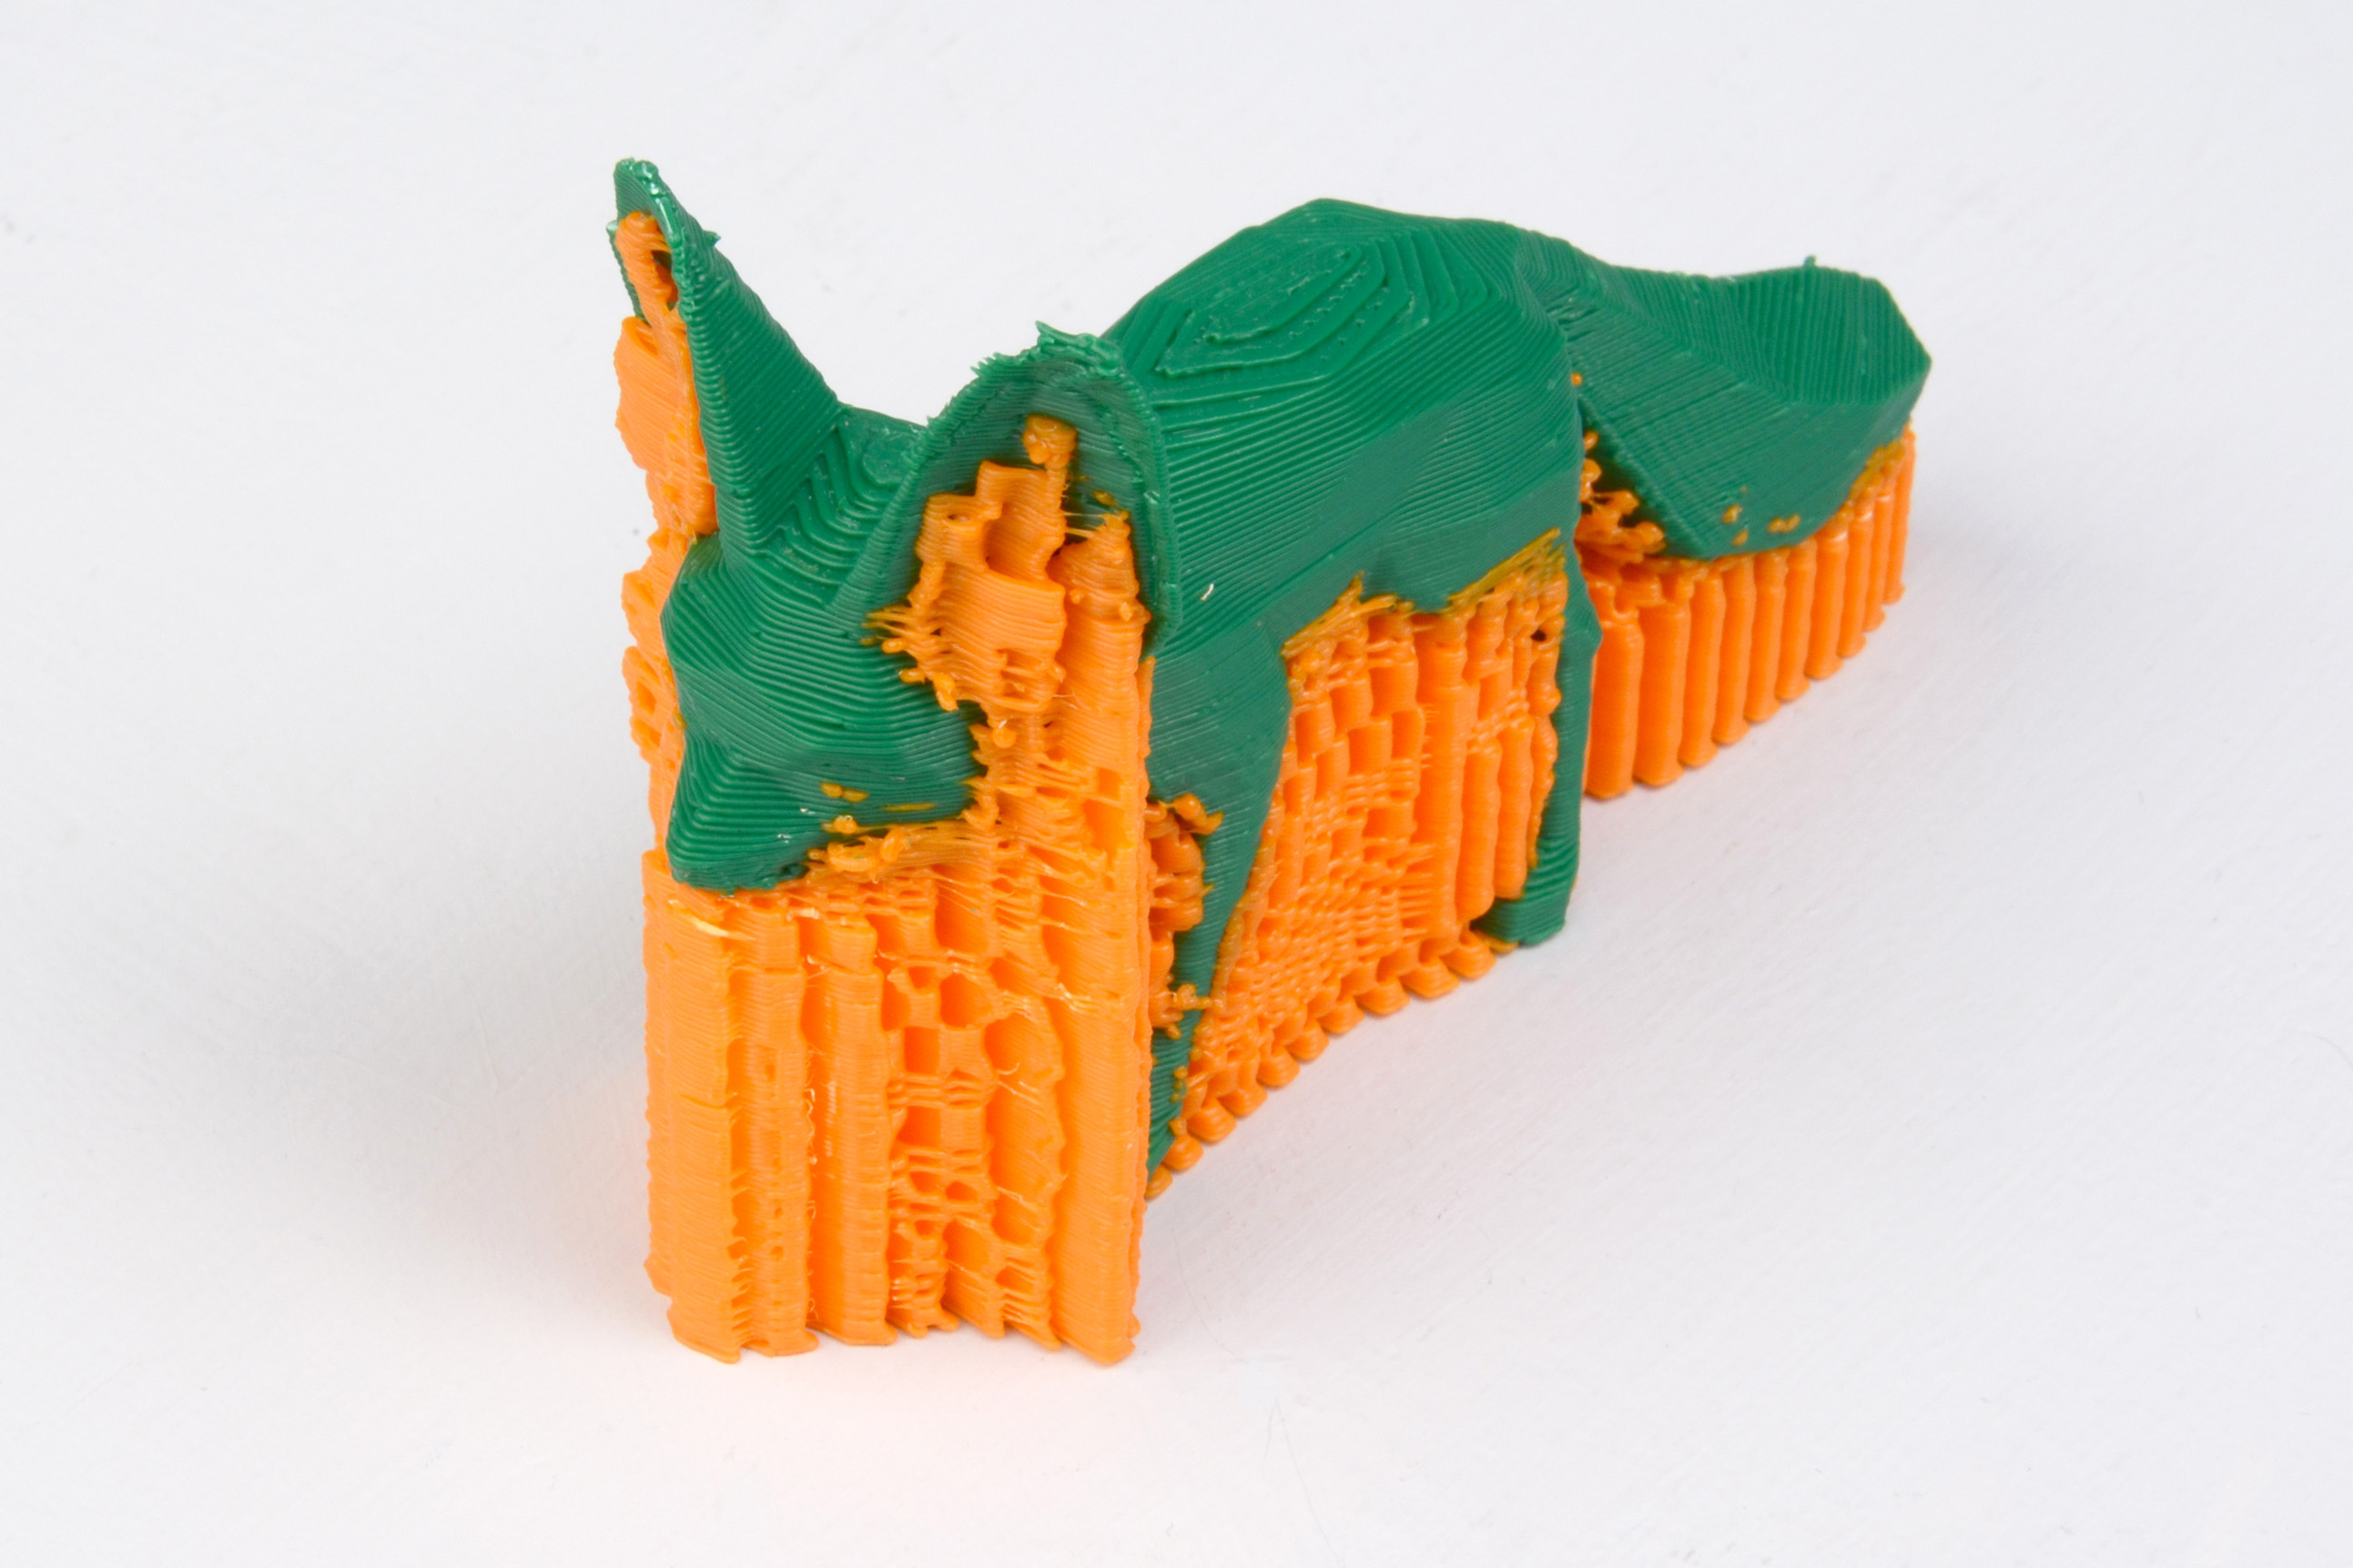
\includegraphics[keepaspectratio=true,width=0.75\textwidth]{simple_mode/support_example.jpg}
\caption{Un exemple d'un objet imprimé avec un support.}
\label{fig:support_example}
\end{figure}

Astuce: Il est parfois utile d'envisager de modifier l'orientation du modèle afin de réduire éventuellement les surplombs.

\index{Print Settings!Support material!Raft layers}
\index{Paramètres d'impression!Support!Radier}
\texttt{Raft layers} (radier) va ajouter des couches supplémentaires sous le modèle et découle depuis les débuts de l'impression 3D. Il peut vous aider à imprimer sans lit chauffé, ou lorsque le lit n'est pas très plat, mais il n'est généralement pas nécessaire et n'est pas recommandé. Le radier nécessite en outre un post-traitement pour le supprimer.
% paragraph support_material (end)

\paragraph{Vitesse. (Speed)} % (fold)
\label{par:simple_speed}
\index{Print Settings!Speed}
En mode simple, il n'y a que trois réglages de vitesse à configurer:
\index{Print Settings!Speed!Perimeters}
\index{Paramètres d'impression!Périmètres}
\index{Print Settings!Speed!Infill}
\index{Paramètres d'impression!Vitesse!Remplissage}
\index{Print Settings!Speed!Travel}
\index{Paramètres d'impression!Vitesse!Déplacement}
\begin{itemize}
	\item \texttt{Perimeters} (Perimeters) - Le contour du modèle peut bénéficier d'une vitesse d'impression légèrement plus lente de sorte que la peau extérieure de l'impression ait moins de défauts.
	\item \texttt{Remplissage} (Infill) - Comme le remplissage est caché il peut être extrudé un peu plus vite. Prenez bien soin de ne pas aller trop vite, car plus la vitesse est élevée, et plus les extrusions sont minces, et cela peut affecter la façon dont se fait la liaison entre les extrusions.
	\item \texttt{Déplacement} (Travel) - Le saut entre la fin d'une extrusion et la suivante doivent généralement être effectuées aussi rapidement que l'imprimante le permet , afin de minimiser les dégâts causés par suintement de matériau depuis la buse.
\end{itemize}
% paragraph speed (end)

\paragraph{Bordure. (Brim)} % (fold)
\label{par:simple_brim}
\index{Print Settings!Brim}
\index{Paramètres d'impression!Bordure}
\index{Print Settings!Brim!Brim width}
\index{Paramètres d'impression!Bordure!Largeur de bordure}
\texttt{Brim width} (largeur de bordure) est utilisé pour ajouter plus de périmètres à la première couche, en tant base supplémentaire, afin de fournir une plus grande surface pour que l'impression colle au lit , afin de réduire les déformation (voir §\ref{sec:the_important_first_layer}). Le bord est ensuite découpée une fois que l'impression est terminée et retirée du lit.

\begin{figure}[H]
\centering
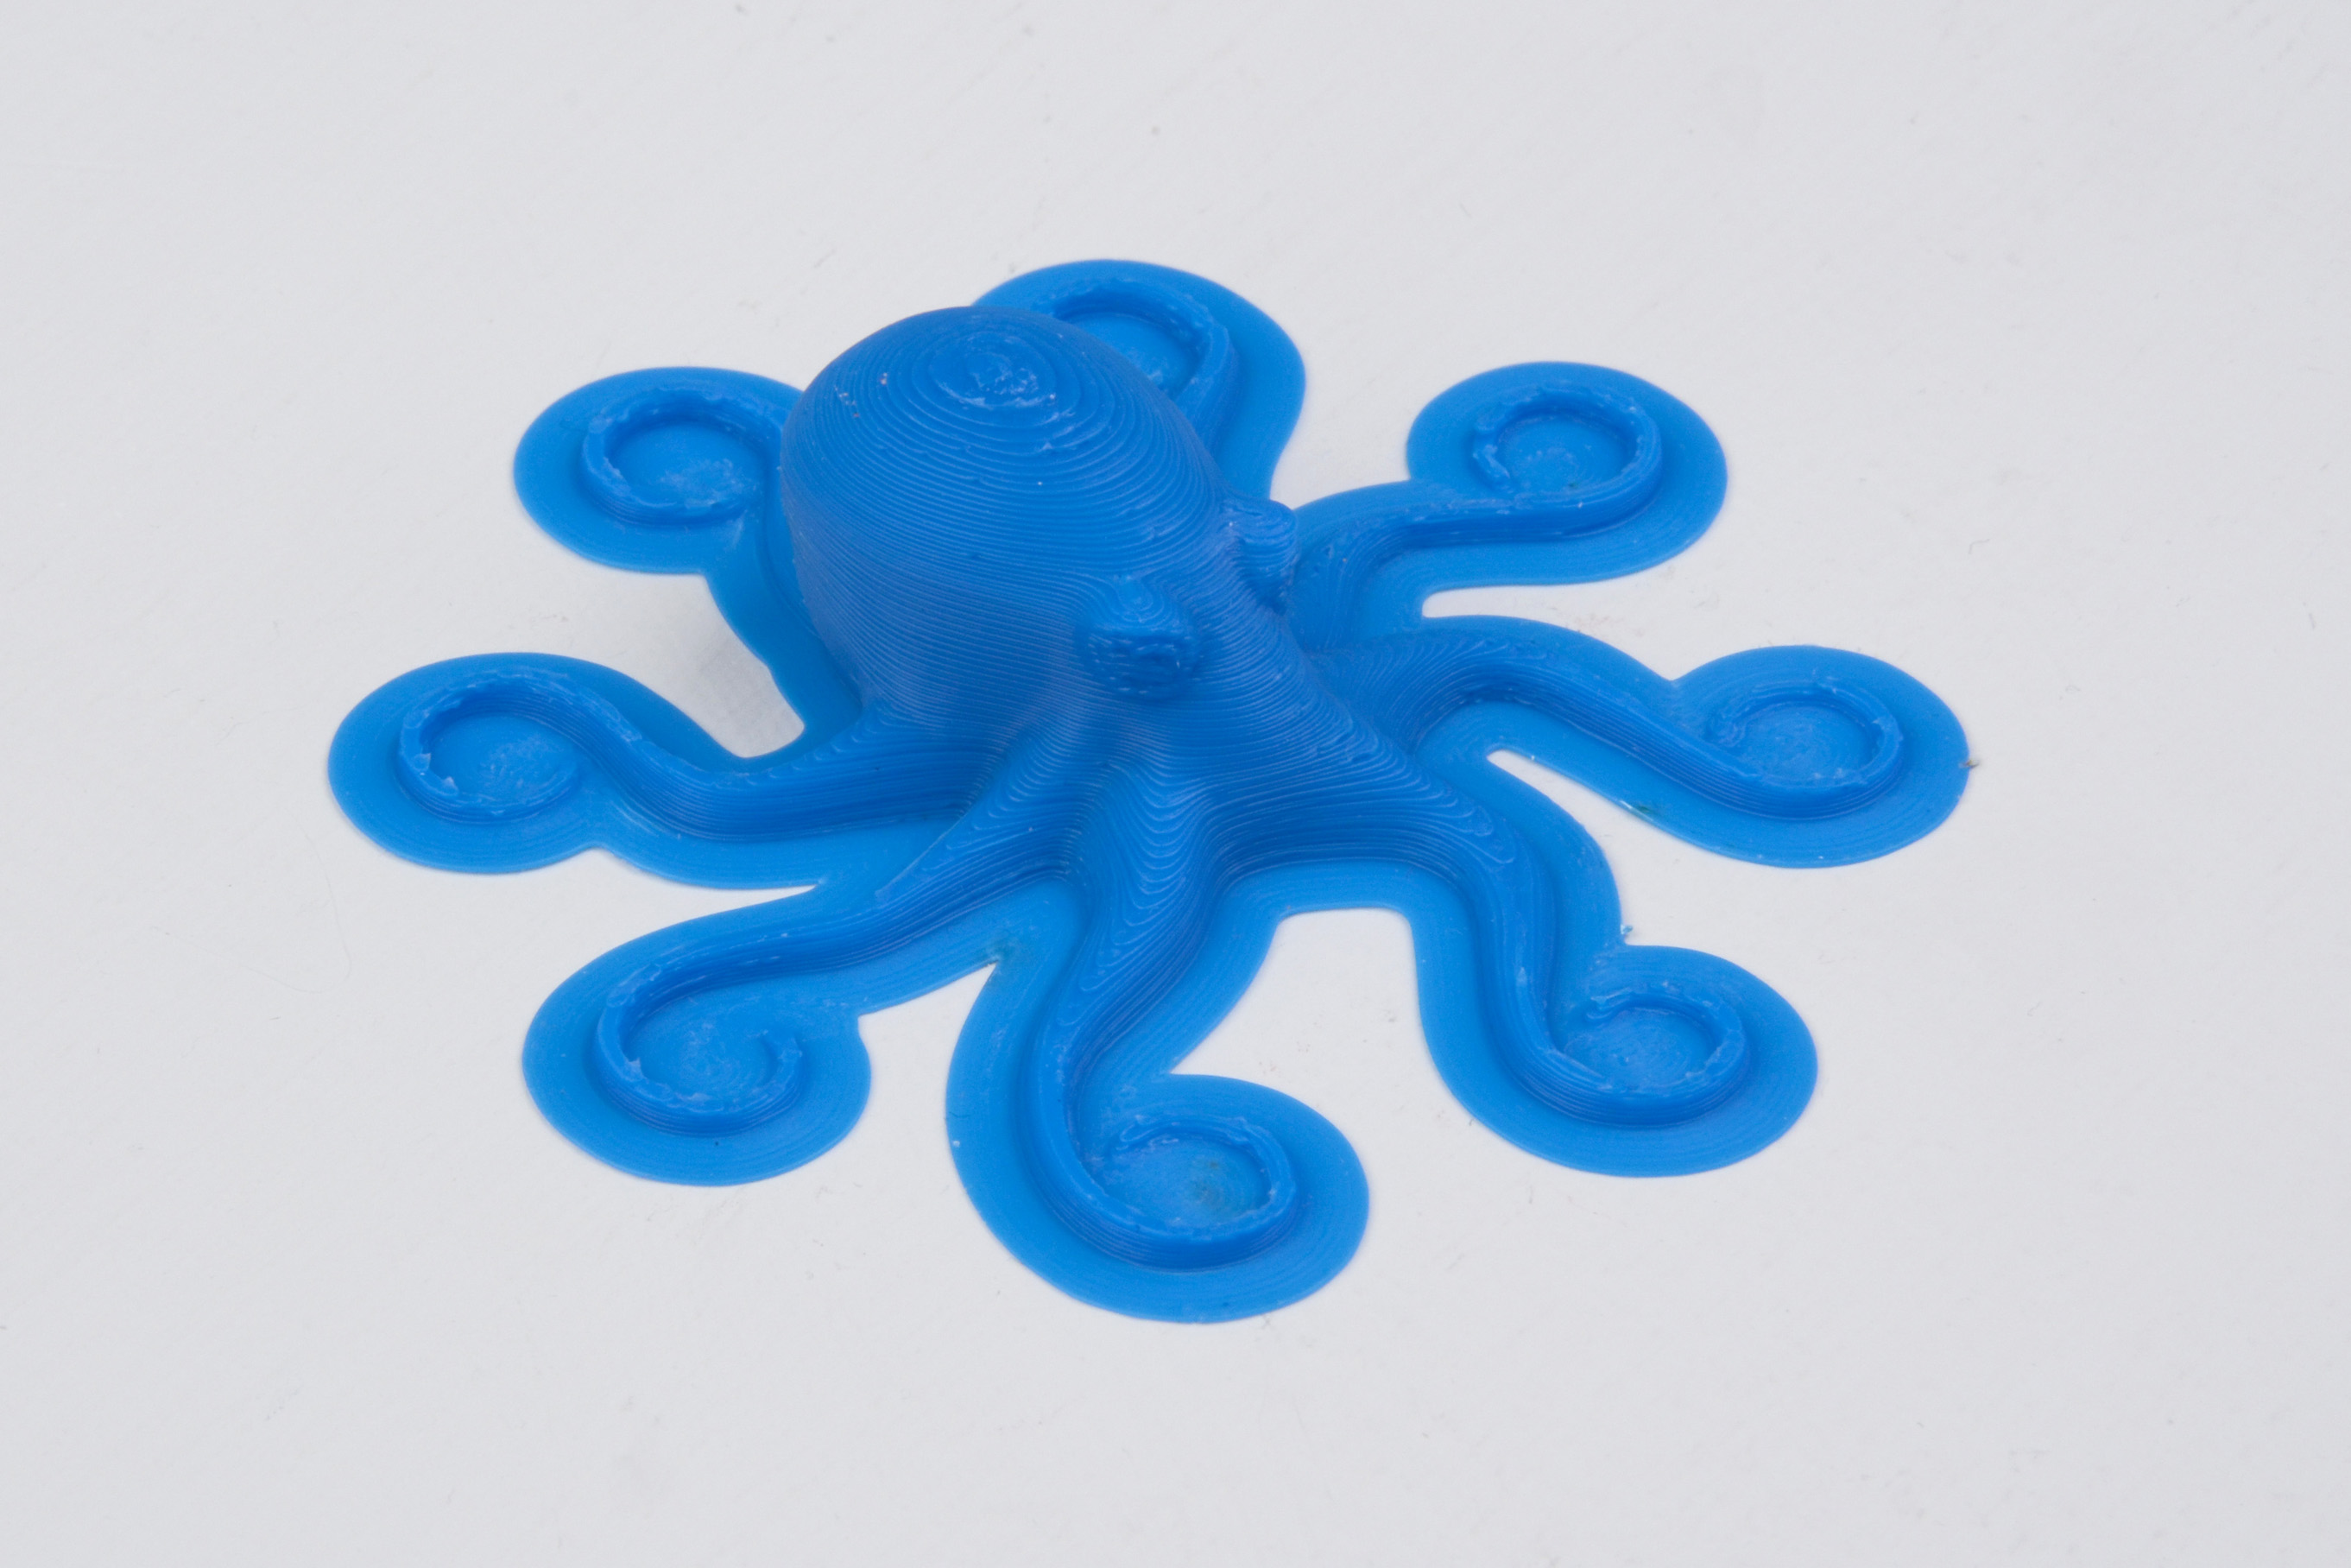
\includegraphics[keepaspectratio=true,width=0.75\textwidth]{simple_mode/brim.jpg}
\caption{Un exemple de bordure.}
\label{fig:an_example_of_brim}
\end{figure}

% paragraph brim (end)

\paragraph{Impression Sequentielle.} % (fold)
\label{par:sequential_printing}
Cette fonction permet de composer un plateau d'objets, mais que l'imprimante compléter chacun individuellement avant de revenir à Z = 0 et en continuant par le suivant. Voir la section sur l'impression séquentielle dans le chapitre des sujets avancés.


\subsection{Filament Settings}
\index{Filament Settings}

The \texttt{Filament Settings} will normally be used infrequently, for example on receipt of a new roll of filament.

\begin{figure}[H]
\centering
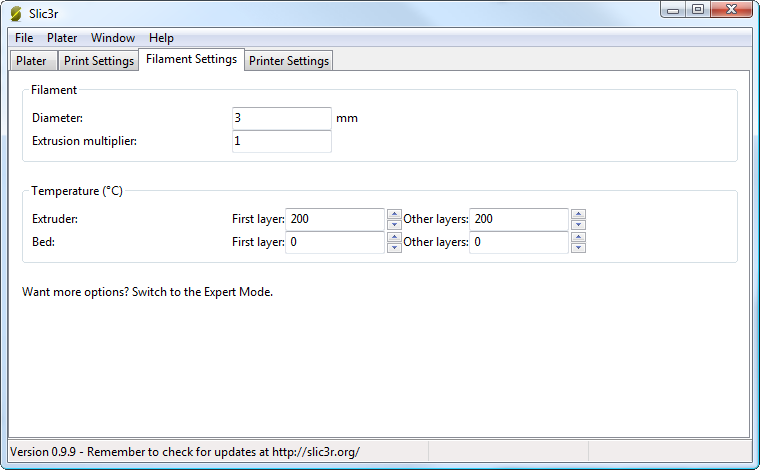
\includegraphics[width=\textwidth]{simple_mode/simple_mode_filament_settings.png}
\caption{Simple Mode: Filament Settings.}
\label{fig:simple_mode_filament_settings}
\end{figure}

\paragraph{Filament.} % (fold)
\label{par:filament}
\index{Filament Settings!Filament}
\index{Filament Settings!Filament!Diameter}
The \texttt{Diameter} setting will already have been filled from the value given during the wizard (see p.\pageref{sub:4_filament_diameter}), but can be updated here.

\index{Filament Settings!Filament!Extrusion multiplier}
The \texttt{Extrusion multiplier} setting allows the fine tuning of the extrusion flow rate, and is is given as a factor, e.g. 1 means 100\%, 1.5 would mean 150\%.  Whilst the value should ideally be set in the firmware it can be useful to test slight changes to the rate by altering this value.  It varies the amount of plastic proportionally and should be changed in very small steps (e.g. +/- 0.05) as the effects are very visible.
% paragraph filament (end)

\paragraph{Temperature.} % (fold)
\label{par:temperature}
\index{Filament Settings!Temperature!Extruder}
\index{Filament Settings!Temperature!Bed}
These values are also filled from the wizard, but here the opportunity exists to set the temperature for the first layer (see p.\pageref{sec:the_important_first_layer}).
% paragraph temperature (end)


\subsection{Printer Settings}
\index{Printer Settings}

The \texttt{Printer Settings} will be updated the least, unless Slic3r is going to be used for many printers, for example, in a 3D printer farm.

\begin{figure}[H]
\centering
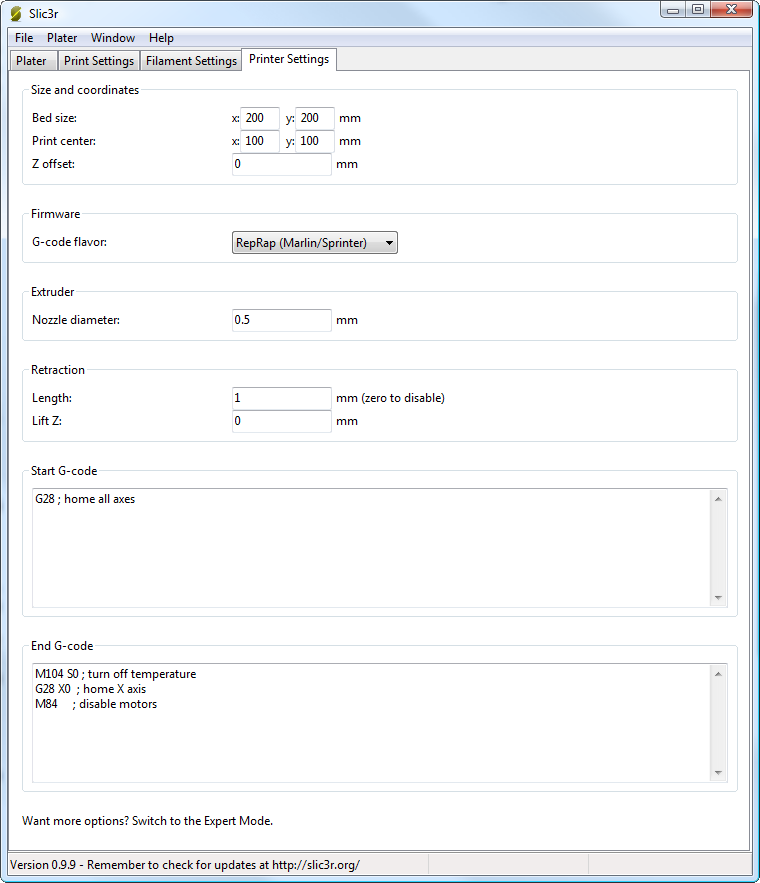
\includegraphics[width=\textwidth]{simple_mode/simple_mode_printer_settings.png}
\caption{Simple Mode: Printer Settings.}
\label{fig:simple_mode_printer_settings}
\end{figure}

\paragraph{Size and coordinates.} % (fold)
\label{par:size_and_coordinates}
\index{Printer Settings!Size and coordinates}
\index{Printer Settings!Size and coordinates!Bed size}
The \texttt{Bed size} setting is taken from the wizard (see p.\pageref{sub:2_bed_size}) and is only used for previewing the model in the plater.

\index{Printer Settings!Size and coordinates!Print center}
The \texttt{Print center} is the point around which the print will be centered.  A \texttt{Bed size} of 200mmx200mm and a \texttt{Print center} of 100mmx100mm would sit the print in the middle.  Should it be desired to print away from the center, because of a scratch in the glass perhaps, then this option should be used.

\index{Printer Settings!Size and coordinates!Z offset}
\texttt{Z offset} can be used to compensate for an incorrectly calibrated Z end-stop.  If the nozzle stops slightly too far from the bed, then adding a negative value will offset all layers by that amount.  The correct solution however is to fix the end-stop itself.

The optimal Z endstop position is where the nozzle tip barely touches the surface of the bed when homed.  A sheet of paper makes a good gauge for this very small distance.  It is not recommended to use this setting to try and improve layer adhesion, by "squashing" the bottom layer into the bed, instead look at the suggestions in section \ref{sec:the_important_first_layer}.
% paragraph size_and_coordinates (end)

\paragraph{Firmware.} % (fold)
\label{par:firmware}
\index{Printer Settings!Firmware!G-code flavour}
As selected in the wizard (see p.\pageref{sub:1_firmware_type}), \texttt{G-code flavour} defines the dialect of G-code generated.
% paragraph firmware (end)


\paragraph{Extruder.} % (fold)
\label{par:extruder}
\index{Printer Settings!Extruder!Nozzle diameter}
\texttt{Nozzle diameter} was defined in the wizard (see p.\pageref{sub:3_nozzle_diameter}).
% paragraph extruder (end)

\paragraph{Retraction.} % (fold)
\label{par:retraction}
\index{Printer Settings!Extruder!Retraction!Length}
Unless the material being extruded has a very high viscosity it may ooze between extrusions due to gravity.  This can be remedied by actively retracting the filament between extrusions.  Setting the \texttt{Length} parameter to a positive value will cause the filament to be reversed by that many millimeters before travel.  The retraction will then be compensated for by the same amount after the travel move, before starting the new extrusion path.

A value of between 1 and 2mm is usually recommended. Bowden extruders may need up to 4 or 5mm due to the hysteresis introduced by the tube.
\index{Printer Settings!Extruder!Retraction!Lift Z}
Setting the \texttt{Lift Z} parameter to a positive value will raise the entire extruder on the Z axis by that many millimeters during each travel.  This can be useful to ensure the nozzle will not catch on any already laid filament, however it is usually not necessary and will slow the print speed.  A value of 0.1mm is usually sufficient.
% paragraph retraction (end)

\paragraph{Start, End and Layer Chance G-codes.} % (fold)
\label{par:start_end_g_code}
\index{Printer Settings!Custom G-code!Start G-code}
\index{Printer Settings!Custom G-code!End G-code}
Custom G-code commands can be run before a print starts and after a print finishes.

Placeholders can be inserted in the G-code commands\footnote{https://github.com/alexrj/Slic3r/wiki/FAQ\#what-placeholders-can-i-use-in-custom-g-code}.  For example [next\_extruder] would return the index of the next extruder.

The RepRap wiki is a good resource to learn about the variety of G-codes available: \texttt{http://reprap.org/wiki/G-code}.

Note: Be sure to check that a given G-code is valid for your firmware.

The codes specified in \texttt{Start G-code} are inserted at the beginning of the output file, directly after the temperature control commands for extruder and bed.  Note that if temperature control commands are specified (M104 and M190) then these will replace the temperature G-codes introduced by the \texttt{Filament} settings.

Some common G-codes to use before the print starts are:
\begin{itemize}
	\item \textbf{G28}  - Homes all the axes.
\end{itemize}


Some common G-codes to use after the print ends are:
\begin{itemize}
	\item \textbf{M104 S0}  - Sets the extruder temperature to zero.
	\item \textbf{M140 S0} - Sets the heated bed temperature to zero.
	\item \textbf{G28 X0} - Home the X axis.
	\item \textbf{M84}  - Disables the motors.
\end{itemize}
% paragraph start_end_g_code (end)

% section simple_mode (end)\section{Simple Mode}
